\section{Anomaly Detection Methods}

\subsection{Different domains and their advantages}
-----Time domain

-----Frequency domain

\subsection{Probabilistic Approach}

\subsection{K Means Clustering}

\begin{figure}[t]
    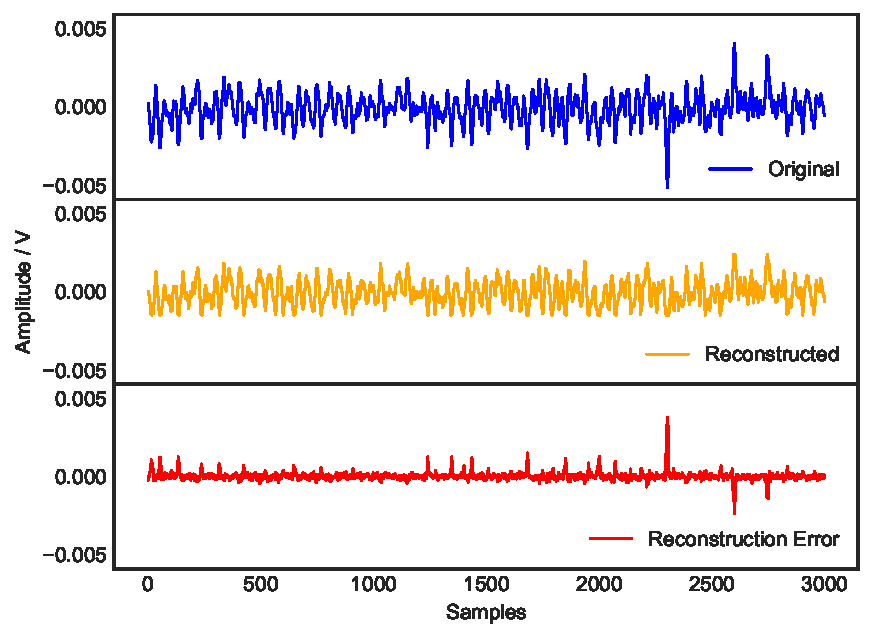
\includegraphics[width=1.0\textwidth]{fig/kmeans.pdf}
    \caption[K mean clustering plot]{Fancy figure goes here.}
    \label{fig:kmeanerror}
\end{figure}

\subsection{LSTM Recurrent Neural Networks}

\begin{figure}[t]
    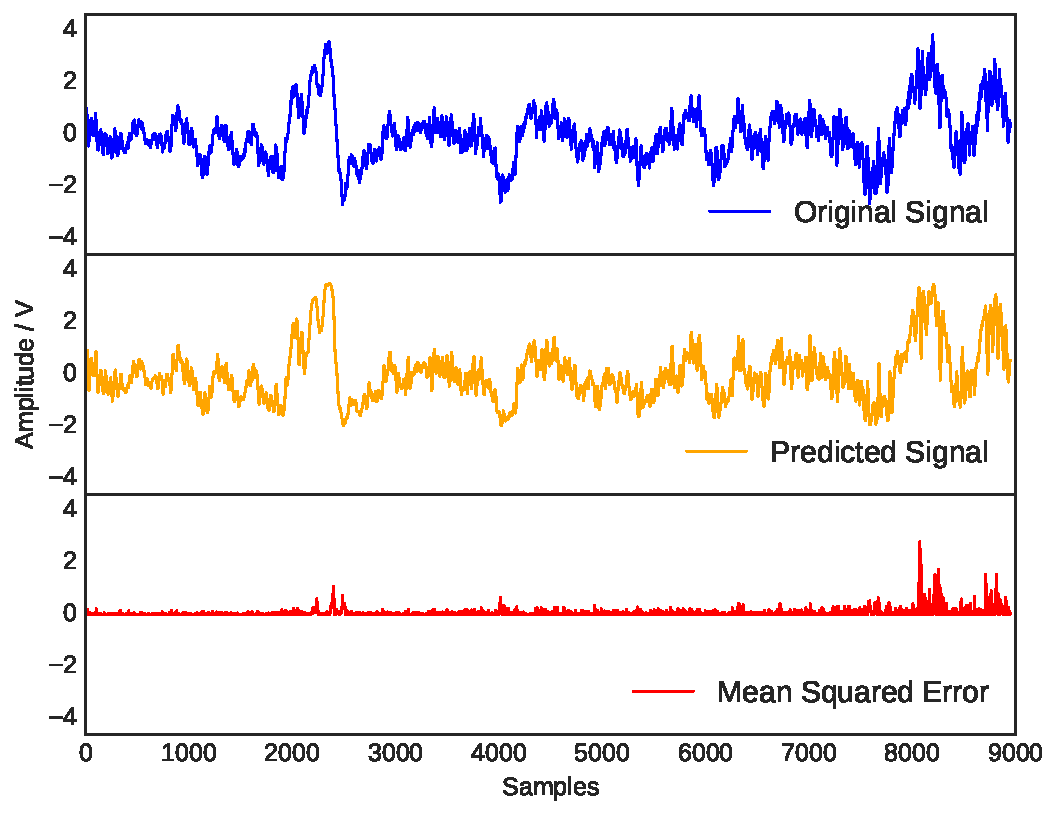
\includegraphics[width=1.0\textwidth]{fig/neuralnetwork.pdf}
    \caption[Neural Network]{Using the LSTM funtionality provided by \texttt{Keras}.}
    \label{fig:kmeanerror}
\end{figure}
